We have implemented a way of color correcting the images given as input. It consists of two parts, where the first part is black balancing and the second part is white balancing. An example of what our algorithm achieve is pictured in Figure \ref{fig:cc}.  

\begin{figure}[H]
\centering

\begin{subfigure}{.33\textwidth}
  \centering
  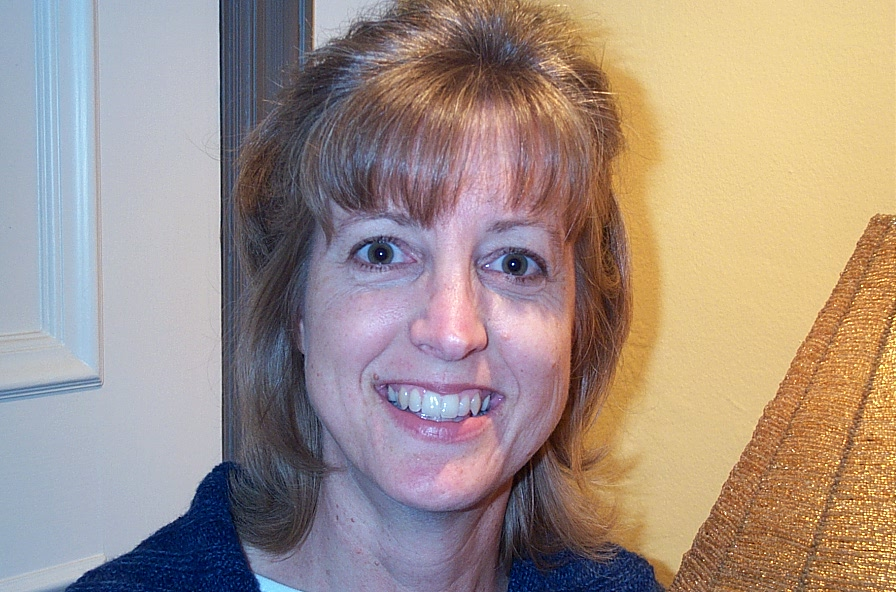
\includegraphics[width=0.95\textwidth]{img/cc/orig.jpg}
  \caption{}
\end{subfigure}%
\begin{subfigure}{.33\textwidth}
  \centering
  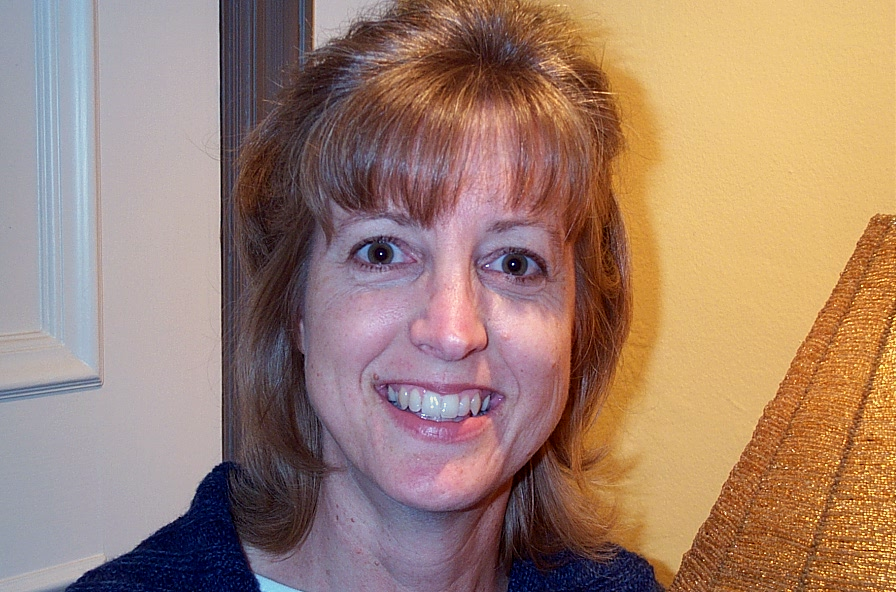
\includegraphics[width=0.95\textwidth]{img/cc/cc.png}
  \caption{}
\end{subfigure}%

\caption{Original image (a) and color corrected image (b).}


\label{fig:cc}
\end{figure}


\subsubsection{Black balancing}
This part aims to calibrate the black pixels of the image in order to make the most black pixels true black. We got the idea to do this when we saw that some of the faces in our dataset were not correctly estimated by our YCbCr color space thresholding. In particular there were some blue tinted images, such as Figure \ref{fig:cc}\textit{a}, that did not register faces properly. 

To solve this problem we extract a few percent ($1.5$) of the most black pixels in each channel of the image. Then, we compute the mean value of these before we subtract the computed values from each pixel of the image. The resulting image will then contain more pure black pixels but also more poor white pixels, which leads us on to the next part, namely white balancing.


\subsubsection{White balancing}
This part aims to calibrate the white pixels of the image in order to achieve better white pixels. It is essentially the same process as black balancing, however with one notable difference. Instead of utilizing subtraction by the mean values we apply scale factors that raise these mean white values of the brightest pixels to become true white. Here we take $0.1$ percent of the most white pixels of each channel into consideration when computing the scale factors.
